\documentclass[10pt,a4paper]{article}
\usepackage{hyperref}
\usepackage[a4paper, total={6in, 10in}]{geometry}
\usepackage[LGR]{fontenc}
\usepackage[utf8]{inputenc}
\usepackage[greek]{babel}
\usepackage{graphicx}
\graphicspath{ {./images/} }

\title{ Γραφική με Υπολογιστές \\ -Εργασία \textlatin{\#}3-}
\author{Θωμάς Πλιάκης \\ \textlatin{tpliakis@ece.auth.gr} \\ AEM: 9018}
\date{\today}

\begin{document}
\maketitle

\section*{\textlatin{ambient\_light}}
Η συνάρτηση \textbf{\textlatin{ambient\_light}} απλά εκτελεί έναν πολλαπλασιαμό μεταξύ μιας σταθεράς και ενός διανύσματος για να υπολογίσει την ένταση της τριχρωματικής ακτινοβολίας του διάχυτου φωτισμού:

\[I = ka * Ia\]   


\section*{\textlatin{diffuse\_light}}
Η συνάρτηση \textbf{\textlatin{diffuse\_light}} για να υπολογίσει την ένταση της τριχρωματικής ακτινοβολίας στην διάχυτη ανάκλαση εκτελεί τα παρακάτω βήματα:

\begin{enumerate}
    \item Υπολογίζει το διανυσμα μεταξύ του σημείου \textbf{\textlatin{P}} και της πηγής του φωτός
    \[\vec{l} = light\_positions - P\]   
    \item Κανονικοποιεί αυτό το διάνυσμα
    \[\hat{L} = \frac{\vec{l}}{||l||}\]
    \item Και τέλος βρίσκει την ακτινοβολία εκτελώντας την πράξη. Υπολογίζοντας το εσωτερικό διάνυσμα μεταξύ του κανονικού διανύσματος και του διανύσματος \textlatin{L}.
    \[I = light\_intensities*color*kd*{\vec{L}}\cdot{\vec{N}}\] 
\end{enumerate}

\section*{\textlatin{specular\_light}}
Η συνάρτηση \textbf{\textlatin{diffuse\_light}} για να υπολογίσει την ένταση της τριχρωματικής ακτινοβολίας στην κατοπτρική ανάκλαση εκτελεί τα παρακάτω βήματα:

\begin{enumerate}
    \item Υπολογίζει το διάνυσμα μεταξύ του σημείου \textbf{\textlatin{P}}  και της πηγής του φωτός και το κανονικοποιεί 
    \[\vec{l} = light\_positions - P\]   
    \[\hat{L} = \frac{\vec{l}}{||l||}\]
    \item Υπολογίζει το διάνυσμα μεταξύ του σημείου \textbf{\textlatin{P}} και του παρατηρητή, δηλαδή της κάμερας, και το κανονικοποιεί 
    \[\vec{v} = cam\_pos - P\]   
    \[\hat{V} = \frac{\vec{v}}{||v||}\]
    \item Και τέλος βρίσκει την ακτινοβολία εκτελώντας την πράξη
    \[I = light\_intensities*color*ks*((2*\vec{N}*({\vec{N}}\cdot{\vec{L}})- \vec{L})\cdot{\vec{V}})^n\]
\end{enumerate}

\section*{\textlatin{calculate\_normals}}
Η συνάρτηση \textbf{\textlatin{calculate\_normals}} υπολογίζει τον πίνακα των κάθετων διανυσμάτων σε κάθε κορυφή με τα παρακάτω βήματα:

\begin{enumerate}
    \item Υπολογίζει το διάνυσμα μεταξύ της πρώτης κορυφής και της δεύτερης και το διάνυσμα της δεύτερης και τρίτης κορυφής και παίρνει το εξωτερικό γινόμενο τους ώστε να βρει το κάθετο διάνυσμα στην επιφάνεια και το κανονικοποιεί. 
    \[\vec{N} = \vec{v01}\times\vec{v12}\]
    \[\hat{N} = \frac{\vec{N}}{||N||}\]
    \item Υπολογίζει έναν πίνακα που αποθηκέυει σε ποια τρίγωνα ανήκει κάθε κορυφή. 
    \item Και τέλος με την βοήθεια του πίνακα αυτού υπολογίζει το κάθετο διάνυσμα στην κάθε κορυφή ως τον μέσο όρο των κάθετων διανυσμάτων των τριγώνων που η κορυφή αυτή συμμετέχει.
\end{enumerate}

\section*{\textlatin{render\_object}}
Ο κώδικας στην συνάρτηση \textbf{\textlatin{render\_object}} περιγράφεται στα παρακάτω βήματα:

\begin{enumerate}
    \item Γίνεται υπολογισμός των κάθετων διανυσμάτων των τριγώνων με την \textbf{\textlatin{calculate\_normals}}.
    \item Γίνεται η προβολή των τριγώνων στις 2 διαστάσεις, μετατρέπονται οι ίντσες της κάμερας σε \textlatin{pixels} και υπολογίζεται το βάθος κάθε κορυφής με την συνάρτηση \textbf{\textlatin{rasterize}} της 2 εργασίας.
    \item Βάφεται το \textlatin{backgroung} της φωτογραφίας.
    \item Δημιουργείται η λίστα με τις 4 φωτογραφίες.
    \item Γίνεται υπολογισμός του βάθους του κάθε τριγώνου και αποθηκέυεται στο διάνυσμα \textbf{\textlatin{Dm}}.
    \item Ταξινομείται ο πίνακας με τα βάθη των κορυφών κατά φθίνουσα σειρά. Με την ίδια σειρά ταξινομείται και ο πίνακας \textbf{\textlatin{faces}}, με την βοήθεια του \textbf{\textlatin{D\_order}} που περίεχει την σειρά που ταξινομήθηκε ο \textbf{\textlatin{Dm}}.
    \item Υπολογίζεται το κάντρο βάρους του τριγώνου στον διάνυσμα \textlatin{bcoords}.
    \item Ανάλογα με ποιο από τα 2 \textbf{\textlatin{mode}} χρησιμοποιήσουμε, επιλέγετε η κατάλληλη συνάρτηση, με \textbf{\textlatin{shader ,["phong" , "gouraud"]}}.
 \end{enumerate}

\section*{\textlatin{shade\_gouraud}}
Η συνάρτηση \textbf{\textlatin{shade\_gouraud}} υπολογίζει τον φωτισμό κάθε κορυφής ενός τριγώνου μέσω των συναρτήσεων της ενότητας Α και στην συνέχεια καλεί την \textbf{\textlatin{shade\_triangle}} της πρώτης εργασίας για να χρωματίσει το τρίγωνο με την μέθοδο \textbf{\textlatin{gouraud}}. Η συνάρτηση γεμίζει με χρώμα τα τρίγωνα 4 διαφορετικών φωτογραφιών όπως ζητούνται στην εκφώνηση, και τις επιστρέφει στην συνάρτηση \textbf{\textlatin{render\_object}} ως μια λίστα.

\section*{\textlatin{shade\_phong}}
Η συνάρτηση \textbf{\textlatin{shade\_phong}} ουσιαστικά είναι η συνάρτηση \textbf{\textlatin{shade\_triangle}} της πρώτης εργασίας αλλά κάθε φορά που θα δώσει χρώμα σε κάποιο σημείο ακολουθεί τα εξής βήματα:

\begin{enumerate}
    \item Υπολογισμός του κάθετου διανύσματος σε κάθε σημείο ως εξής:
    \subitem - Αν το τρίγωνο είναι σημείο υπολογίζεται ως ο μέσος όρος των κάθετων διανυσμάτων των κορυφών.
    \subitem - Σε κάθε άλλη περίπτωση ως γραμμική παρεμβολή μεταξύ των κορυφών ή των ενεργών σημείων που αυτό βρίσκεται. Τα κάθετα διανύσματα στα ενεργά σημεία υπολογίζονται με γραμμική παρεμβολή των αντίστοιχων κορυφών που βρίσκονται ανάμεσα.
    \item Υπολογισμός του χρώματος του σημείου με παρόμοιο τρόπο όπως τα κάθετα διανύσματα.
    \item Υπολογιμός του φωτισμού με τις συναρτήσεις της ενότητας Α και τον αντίστοιχων κάθετων διανυσμάτων και χρωμάτων που υπολογίστηκαν για κάθε σημείο.
 \end{enumerate}
 
Δηλαδή δεν έπρεπε να γίνει καμιά αλλαγή στο προς βρίσκουμε τα σημεία που βρίσκονται πάνω ή μέσα στο κάθε τρίγωνο, απλά έπρεπε να γίνει προσθήκη όλων των γραμμικών παρεμβολών.
Επίσης δημιουρηθηκε μια λίστα με 4 φωτογραφίες όπως ζητήθηκε στην εκφώνηση παρόμοια με την συνάρτηση \textbf{\textlatin{shade\_gouraud}}.\\
\\

Στο τέλος πραθέτω τις συναρτήσεις από τις προηγούμενες εργασίες που χρησιμοποίησα:

\section*{Σχόλια}
\begin{itemize}
  \item Τα αποτελέσματα στην συνάρτηση \textbf{\textlatin{shade\_gouraud}} είναι ικανοποιητικά αλλά στην συνάρτηση \textbf{\textlatin{shade\_phong}} είναι λάθος. Για κάποιο λόγο που δεν μπόρεσα να βρω δεν χρωματίζονται σωστά τα τριγώνα αν και προσπάθησα να μην αλλάξω την διαδικασία πλήσρωσης του τριγώνου.
  \item Η μόνη παραδοχή που έγινε ήταν στην δημιουργία των λιστών των 4 φωτογρφιών για κάθε συνάρτηση ώστε να καταφέρω να τις δημιουργήσω τρέχοντας μόνο το αρχείο \textlatin{demo.py} ώστε να μην πειράζω τον κώδικα για κάθε εικόνα.
  \item Χρειάστηκαν περίπου 6  λέπτα για να παραχούν όλες οι εικόνες στον υπολογιστή μου.
\end{itemize}

\section*{Αποτελέσματα για \textlatin{gouraud(ambient,diffuse,specular,all3together)}:} 

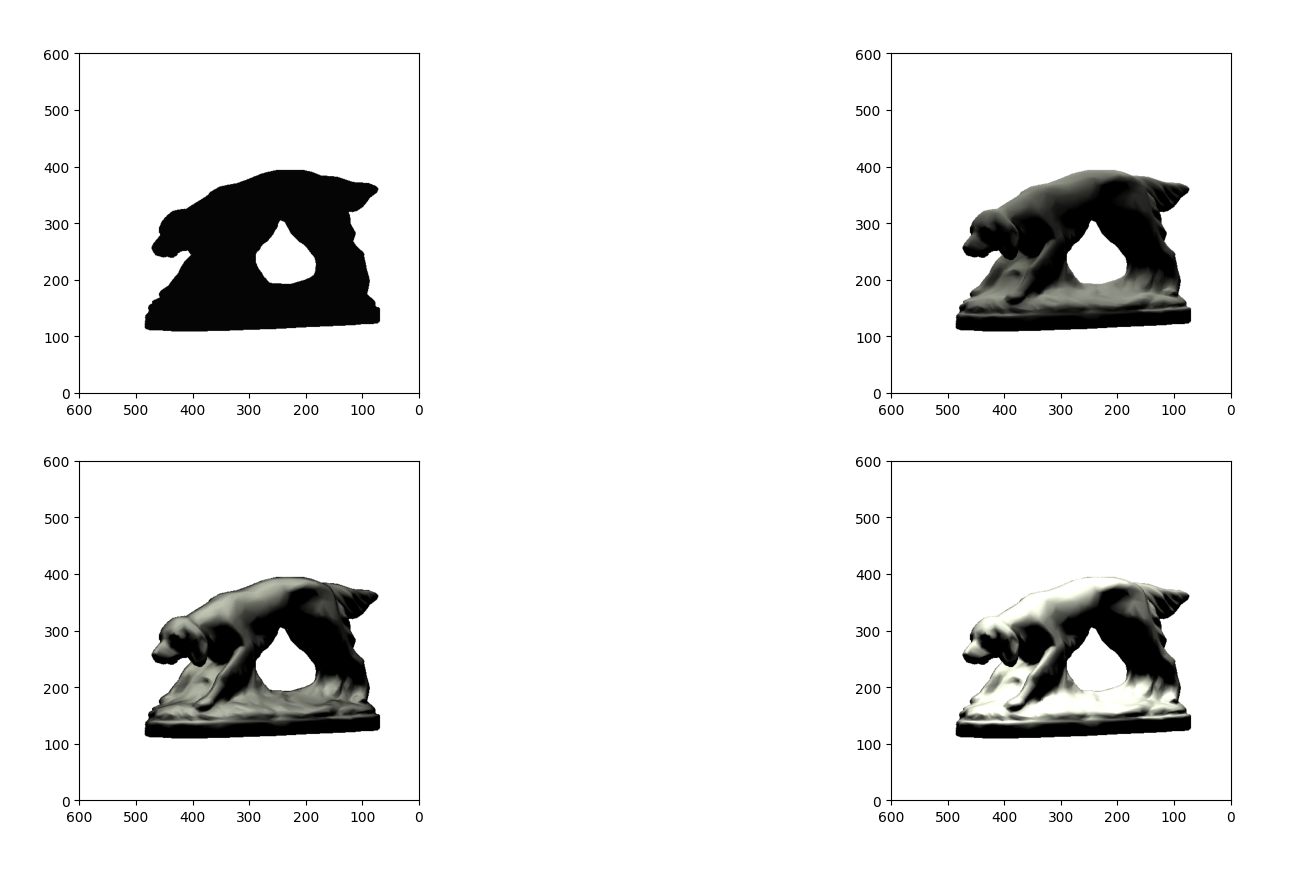
\includegraphics[scale=0.35]{gouraud.png}

\section*{Αποτελέσματα για \textlatin{phong(ambient,diffuse,specular,all3together)}:} 
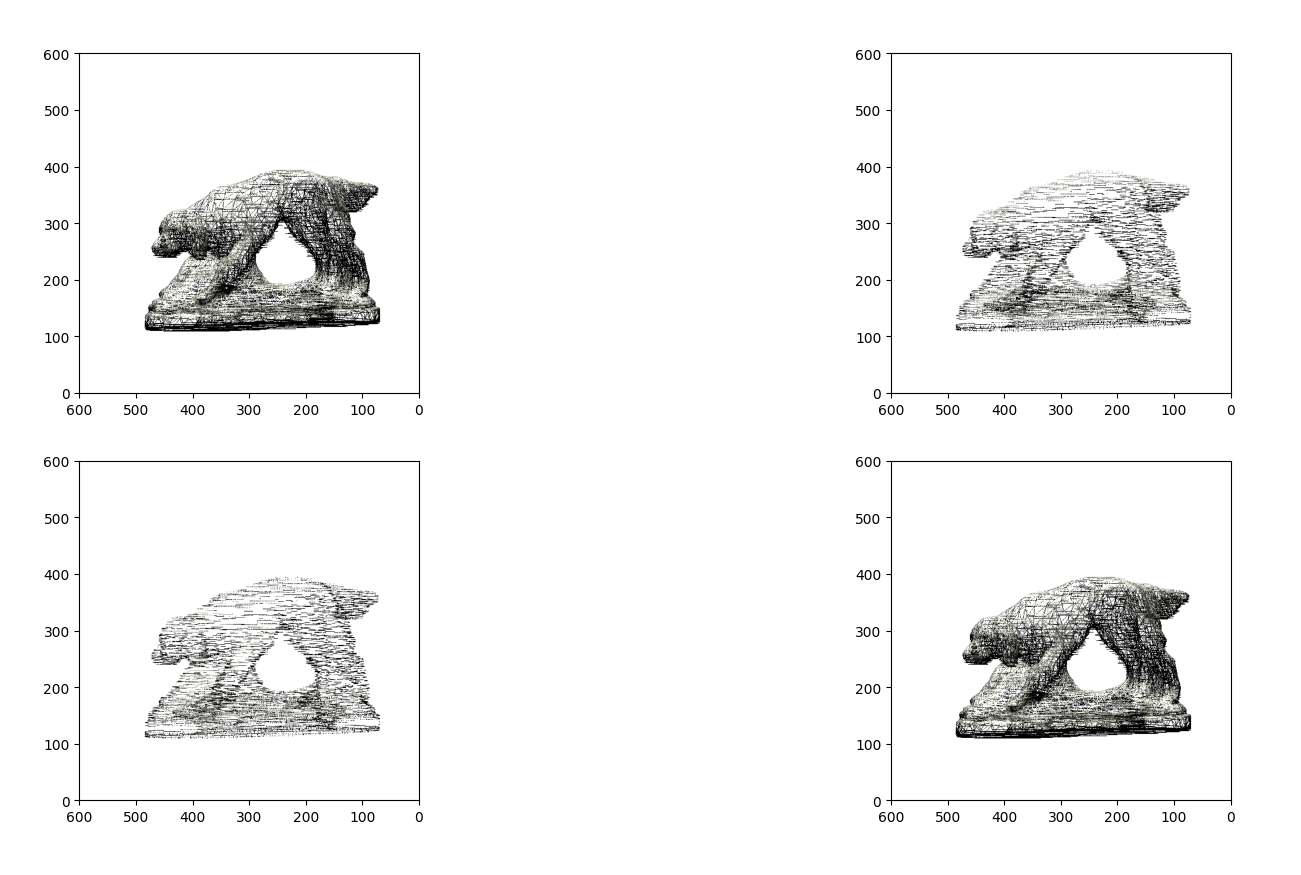
\includegraphics[scale=0.35]{phong.png}

\section*{\textlatin{interpolate\_color}}
Η συνάρτηση \textbf{\textlatin{vector\_interp}} υλοποιεί πολύ απλά μια γραμμική παρεμβολή μεταξύ των σημείων που δίνονται ως ορίσματα με τον παρακάτω τρόπο:

\[r1 = ||x2-x||\]   
\[r2 = ||x-x1||\]
\[percent = \frac{r1}{r1 +r2}\]
\[value = percent*C1+(1-percent)*C2\]

Όπου \textlatin{r1} και \textlatin{r2} είναι οι απόστασεις των ενεργών σημείων από το σημείο της παρεμβολής, \textlatin{r1 + r2} είναι η απόσταση των σημείων \textlatin{x1}, \textlatin{x2}. Με την διαίρεση γίνεται μια κανονικοποίηση για να έχουμε το ποσοστό μεταξύ 0 και 1 που πρέπει να συμμετέχει κάθε σημείο στον χρωματισμό. 

Ο κώδικας, λόγω της βιβλιοθήκης \textbf{\textlatin{numpy}} μπορεί να υλοποιεί την γραμμική παρεμβολή με μεταβλητές οποιονδήποτε διαστάσεων.


\section*{\textlatin{shade\_triangle}}
Επειδή η υλοποίηση των δύο \textbf{\textlatin{mode ,["flat" , "gouraud"]}}, ξεκίνησε διαφορετκά, η ενοποιήση των 2 διαδικασιών έγινε με ένα \textbf{\textlatin{if ... else}} ανάλογα το όρισμα \textbf{\textlatin{shade\_t}}.

Η συνάρτηση \textbf{\textlatin{shade\_triangle}} με όρισμα \textbf{\textlatin{shade\_t = "flat"}} αποδίδει ένα χρώμα σε κάθε τρίγωνο, τον μέσο όρο των χρωμάτων των κορυφών του. Τα βήματα του αλγορίθμου περιγράφονται παρακάτω: 
\begin{enumerate}
    \item Υπολογισμός και αποθήκευσή του μέσου όρου των χρωμάτων στον 1\textlatin{x}3 πίνακα \textbf{\textlatin{c}}.
    \item Υπολογισμός των ελάχίστων και μεγίστων συντεταγμένων της κάθε πλευράς,  καθώς και της κλίσης τους, \textbf{\textlatin{Ykmin,Xkmin,Ykmax,Xkmax}}.
    \item Εύρεση των ολικών μεγίστων και ελαχίστων συντεταγμένων του τριγώνου, \textbf{\textlatin{Ymin,Xmin,Ymax,Ymin}}.
    \item Βρίσκουμε ποιες είναι οι αρχικές ενεργές πλευρές(παίρνουν το λογικό 1) και αποθηκεύουμε σε πίκανκα τις συντεταγμένες τους, που αποτελούν και τα ενεργά οριακά τους σημεία \textbf{\textlatin{ActiveSides,Xk}}. Στον πίνακα \textbf{\textlatin{Xact}} αποθηκεύονται οι τετμημένες των 2 ενεργών σημείων μόνο.
    \item Μπαίνουμε στην κυρίως επανάληψη στην οποία:
    \begin{itemize}
        \item Ελέγχουμε αν βρισκόμαστε σε κορυφή του τριγώνου.
        \item Υλοποιείται το σκανάρισμα σε όλες τις τετμημένες για συγκεκριμένη τεταγμένη κατά την οποία αν κάποιο \textbf{\textlatin{pixel}} βρίσκεται μέσα ή πάνω στο τρίγωνο χρωματίζεται.
        \item Ενημερώνεται η λίστα των ενεργών πλεύρων.
        \item Τέλος ενημερώνεται η λίστα με τα νέα ενεργά σημεία ανάλογα με την κλίση της κάθε πλευράς του τριγώνου.
      \end{itemize}
  \end{enumerate}


H συνάρτηση \textbf{\textlatin{shade\_triangle}} με όρισμα \textbf{\textlatin{shade\_t = "gouraud"}} έκτελεί τις ίδιες αρχικοποιήσεις με προηγουμένως αλλά και κάποιες ακόμα. Τα επιπλέον βήματα του αλγορίθμου που γίνονται είναι:
\begin{enumerate}
    \item Αποθηκεύση των δεικτών των κορυφών κάθε ακμής στις λίστες \textbf{\textlatin{minindex, maxindex}}.
    \item Αποθηκεύση των δεικτών των 2 ενεργών σημείων κάθε ακμής στις λίστα \textbf{\textlatin{index}} για προσέλαση των \textbf{\textlatin{colorsAct}}, \textbf{\textlatin{Xact}} πινάκων.
    \item Αποθηκεύση του χρώματος των ενεργών οριακών σημείων στην λίστα  \textbf{\textlatin{colorsAct}}.
    \item Όταν γίνεται ο χρωματσμός κάποιου σημείου εσωτερικά του τριγώνου, υπολογίζεται το χρώμα του από την \textbf{\textlatin{interpolate\_color}} και τα 2 ενεργά σημεία. 
    \item Ο υπολογισμός του χρώματος για τα ενεργά οριακά σημεία γίνεται με χρήση της \textbf{\textlatin{interpolate\_color}} από τις αντίστοιχες κορυφές κατά την ενημέρωση της λίστας με τα ενεργά σημεία.
\end{enumerate}

Όλα τα παραπάνω γίνονται για τον χρωματισμό ενός αντικειμένου
ολόκληρου που αποτελείται από πολλά τρίγωνα. Αυτό γίνεται στην συνάρτηση:

\section*{\textlatin{affine\_transform}}

Η πρώτη συνάρτηση εκτελεί τον μετασχηματισμό \textlatin{affine}. Πρώτα κατασκευάζει τον πίνακα
περιστροφής με βάση την φόρμουλα του \textlatin{Rodrigues} μετά κατασκευάζει τον πίνακα μετασχηματισμού και
στην συνέχεια γίνεται ο υπολογισμός με ομογενείς συντεταγμένες.


\section*{\textlatin{system\_transform}}
Αυτή η συνάρτηση αλλάζει το σύστημα συντεταγμένων των σημείων που δίνονται με βάση των
πίνακα στροφής που δίνεται. Πρώτα δημιουργείται ο πίνακας μετασχηματισμού και μετά οι
συντεταγμένες των κορυφών μετατρέπονται σε ομογενείς συντεταγμένες για να γίνουν οι πράξεις.

\section*{\textlatin{project\_cam}}

Η συνάρτηση αυτή «φωτογρφίζει» το αντικείμενο. Πρώτα γίνεται η αλλαγή συστήματος
συντεταγμένων με την προηγούμενη συνάρτηση των σημείων απο το \textlatin{WCS} στο σύστημα της κάμερας.
Στην συνέχεια υπολογίζουμε την απόσταση από την κάμερα και με βάση την προοπτική προβολή οι
3διάστατες συντεταγμένες του γίνονται 2 διαστάσεων με πολλαπλασιαμό με την μεταβλήτη f και
διαίρεση με το βάθος.

\section*{\textlatin{project\_cam\_lookat}}

Εδώ υπολογίζονται τα μοναδιαία διανύσματα του πλαισιού της κάμερας τα οποία τα περνάμε
στην προηγούμενη συνάρτηση ώστε να μπορέσει να στοχεύσει σωστά το αντικείμενο προς
φωτογράφιση.

\section*{\textlatin{rasterize}}
Η συνάρτηση αυτή ελέγχει αν όλα τα σημεία βρίσκονται μέσα στο πλάνο μας, ελέγχοντας αν οι
διαστάσεις τους βρίσκονται μέσα στα εύρη (-\textlatin{camw}/2, \textlatin{camw}/2) στον οριζόντιο άξονα και (-\textlatin{camh}/2,
\textlatin{camh}/2) στον κάθετο, μετακινεί την αρχή της εικόνας κάτω αριστερά και τέλος μετατρέπει τις ίντσες τους
πετάσματος της κάμερας σε ακέραιες θέσεις (\textlatin{pixels}) της εικόνας διαιρώντας τις συνολικές ιντσές προς τα
συνολικά pixels για να πάρουμε την κλίμακα μετατροπής. Με την κλίμακα αυτή μπορούμε να βρούμε τα
\textlatin{pixel} των επιμέρους κορυφών με μια διαίρεση και με την συνάρτηση \textlatin{ceil} της \textlatin{numppy} για να γίνουν
ακέραια.
\end{document}